\documentclass[12pt]{article}
\usepackage{latexsym,amssymb,amsmath} % for \Box, \mathbb, split, etc.
% \usepackage[]{showkeys} % shows label names
\usepackage{cite} % sorts citation numbers appropriately
\usepackage{path}
\usepackage{url}
\usepackage{verbatim}
\usepackage{graphicx}
\usepackage{array}
\usepackage{multirow}

% horizontal margins: 1.0 + 6.5 + 1.0 = 8.5
\setlength{\oddsidemargin}{0.0in}
\setlength{\textwidth}{6.5in}
% vertical margins: 1.0 + 9.0 + 1.0 = 11.0
\setlength{\topmargin}{0.0in}
\setlength{\headheight}{12pt}
\setlength{\headsep}{13pt}
\setlength{\textheight}{625pt}
\setlength{\footskip}{24pt}

\renewcommand{\textfraction}{0.10}
\renewcommand{\topfraction}{0.85}
\renewcommand{\bottomfraction}{0.85}
\renewcommand{\floatpagefraction}{0.90}
\usepackage{graphicx}
\usepackage{wrapfig}
\usepackage{lscape}
\usepackage{rotating}
\usepackage{epstopdf}
\makeatletter
\setlength{\arraycolsep}{2\p@} % make spaces around "=" in eqnarray smaller
\makeatother

% change equation, table, figure numbers to be counted inside a section:
\numberwithin{equation}{section}
\numberwithin{table}{section}
\numberwithin{figure}{section}

% begin of personal macros
\newcommand{\half}{{\textstyle \frac{1}{2}}}
\newcommand{\eps}{\varepsilon}
\newcommand{\myth}{\vartheta}
\newcommand{\myphi}{\varphi}
\usepackage[utf8]{inputenc}

% Default fixed font does not support bold face
\DeclareFixedFont{\ttb}{T1}{txtt}{bx}{n}{8} % for bold
\DeclareFixedFont{\ttm}{T1}{txtt}{m}{n}{8}  % for normal

% Custom colors
\usepackage{color}
\definecolor{deepblue}{rgb}{0,0,0.5}
\definecolor{deepred}{rgb}{0.6,0,0}
\definecolor{deepgreen}{rgb}{0,0.5,0}
\definecolor{backcolour}{rgb}{0.96,0.96,0.96}

\usepackage{listings}

% cpp style for highlighting
\newcommand\cppstyle{\lstset{
		language=C++,
        basicstyle=\tiny\ttfamily,
		keywordstyle=\color{blue}\ttfamily,
		stringstyle=\color{red}\ttfamily,
		commentstyle=\color{green}\ttfamily,
		morecomment=[l][\color{magenta}]{\#},
		frame=tb,                         % Any extra options here
showstringspaces=false,            % 
backgroundcolor=\color{backcolour}
}}


% cpp environment
\lstnewenvironment{cpp}[1][]
{
	\cppstyle
	\lstset{#1}
}
{}

% cpp for external files
\newcommand\cppexternal[2][]{{
		\cppstyle
		\lstinputlisting[#1]{#2}}}

% cpp for inline
\newcommand\cppinline[1]{{\cppstyle\lstinline!#1!}}

\newcommand{\IN}{\mathbb{N}}
\newcommand{\IZ}{\mathbb{Z}}
\newcommand{\IQ}{\mathbb{Q}}
\newcommand{\IR}{\mathbb{R}}
\newcommand{\IC}{\mathbb{C}}
\newcommand{\Real}[1]{\mathrm{Re}\left({#1}\right)}
\newcommand{\Imag}[1]{\mathrm{Im}\left({#1}\right)}
\usepackage{booktabs}
\usepackage{caption}
\usepackage{float}
\usepackage{titlesec}
\usepackage{capt-of}
%dashed line
\usepackage{array}
\usepackage{arydshln}
\setlength\dashlinedash{0.2pt}
\setlength\dashlinegap{1.5pt}
\setlength\arrayrulewidth{0.3pt}

%Widows & Orphans & Penalties

\widowpenalty500
\clubpenalty500
\clubpenalty=9996
\exhyphenpenalty=50 %for line-breaking at an explicit hyphen
\brokenpenalty=4991
\predisplaypenalty=10000
\postdisplaypenalty=1549
\displaywidowpenalty=1602
\floatingpenalty = 20000
\usepackage[T1]{fontenc}
\usepackage{fontspec}
\setmainfont[Scale=0.85, Ligatures={Required,Common,Contextual,TeX}]{TeX Gyre Schola} % Incredible font inside latex


\newcommand{\norm}[2]{\|{#1}\|_{{}_{#2}}}
\newcommand{\abs}[1]{\left|{#1}\right|}
\newcommand{\ip}[2]{\left\langle {#1}, {#2} \right\rangle}
\newcommand{\der}[2]{\frac{\partial {#1}}{\partial {#2}}}
\newcommand{\dder}[2]{\frac{\partial^2 {#1}}{\partial {#2}^2}}
\usepackage{enumitem}
\newcommand{\nn}{\mathbf{n}}
\newcommand{\xx}{\mathbf{x}}
\newcommand{\uu}{\mathbf{u}}
\usepackage{tikz}
\usetikzlibrary{arrows}
\usetikzlibrary{positioning}
\usepackage{titlesec}
\newcommand{\junk}[1]{{}}
\usepackage{sectsty}
\usepackage{xcolor}

\newcommand\MyBox[2]{
	\fbox{\lower0.75cm
		\vbox to 1.7cm{\vfil
			\hbox to 1.7cm{\hfil\parbox{1.4cm}{#1\\#2}\hfil}
			\vfil}%
	}%
}

\makeatletter
\renewcommand*\env@matrix[1][\arraystretch]{%
	\edef\arraystretch{#1}%
	\hskip -\arraycolsep
	\let\@ifnextchar\new@ifnextchar
	\array{*\c@MaxMatrixCols c}}
\makeatother

\makeatletter
\renewcommand*\env@matrix[1][*\c@MaxMatrixCols c]{%
	\hskip -\arraycolsep
	\let\@ifnextchar\new@ifnextchar
	\array{#1}}
\makeatother

\definecolor{darkblue}{rgb}{0,0,0.4}
\usepackage[colorlinks = true,
linkcolor = darkblue,
urlcolor  = darkblue,
citecolor = darkblue,
anchorcolor = darkblue]{hyperref}
% set two lengths for the includegraphics commands used to import the plots:
\newlength{\fwtwo} \setlength{\fwtwo}{0.45\textwidth}
% end of personal macros

\begin{document}
\DeclareGraphicsExtensions{.jpg}

\begin{center}
\textsc{\Huge Multi-core Programming} \\[2pt]
	\textsc{\Large Assignment 5}\\
	\vspace{0.5cm}
  Ali Gholami \\[6pt]
  Department of Computer Engineering \& Information Technology\\
  Amirkabir University of Technology  \\[6pt]
  \def\UrlFont{\em}
  \url{https://aligholamee.github.io}\\
\href{mailto:aligholami7596@gmail.com}{\textit{aligholami7596@gmail.com}}
\end{center}

\begin{abstract}
In this report, we'll analyze the \textit{prefix-sum} (\textit{scan}) problem. There are many uses for scan, including, but not limited to, sorting, lexical analysis, string comparison, polynomial evaluation, stream compaction, and building histograms and data structures (graphs, trees, and so on) in parallel. There are also multiple solutions and algorithms to compute the prefix sum of an array. Sources for this report are provided in the \textit{src} folder. 
\end{abstract} 

\subparagraph{Keywords.} \textit{}

\section{Hillis \& Steele Algorithm}
\subsection{How it works?}
Recall that in each step, we had to add up the elements of the array until now and replace the current element with the addition result. The sequential implementation takes exactly \textit{n} operations (\textit{n is the size of the array}) to complete. The \textit{Hillis \& Steele} algorithm, provides a simple and intuitive parallelization trick using \textit{addition} as a \textit{binary operator} which takes only two arguments. The idea is parallel in theory but it has some problems in practice. Figure 1.1 demonstrates this algorithm better.
\begin{figure}[!h]\centering
	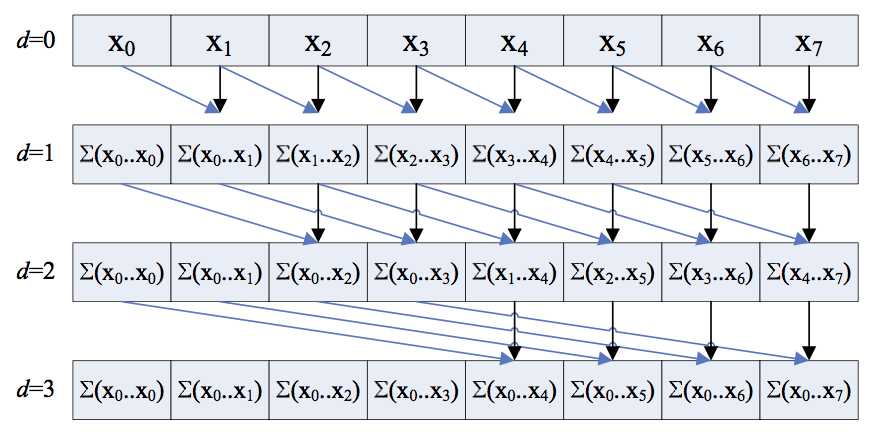
\includegraphics[width=0.7\textwidth]{1_1.png}
	\caption{Demonstration of \textit{Hillis \& Steele} Algorithm.}
	\label{pl1}
\end{figure}

\subsection{Assumptions}
This algorithm assumes that there are as many as processors as data elements. The programmer must divide the computation among a number of thread blocks that each scans a portion of the array on a single multiprocessor of the GPU. Even still, the number of processors in a multiprocessor is typically much smaller than the number of threads per block, so the hardware automatically partitions the \textit{for all} statement into small parallel batches (called warps) that are executed sequentially on the multiprocessor. Because not all threads run simultaneously for arrays larger than the warp size, this algorithm will not work, because it performs the scan in place on the array. The results of one warp will be overwritten by threads in another warp.

\subsection{Work Efficiency}
Even if this algorithm works in some cases, it is not \textit{work efficient}. The minimum number of addition operations needed in the sequential algorithm was \textit{n}. In this algorithm, this number increases to $n\log n$. That's the main reason we call the \textit{Hillis \& Steele} algorithm a \textit{work inefficient} algorithm.
\subsection{Pseudocode}
\begin{cpp}
	1: for d = 1 to log2 n do
	2:     for all k in parallel do
	3:          if k >= power(2, d)  then
	4:              x[k] = x[k – power(2, d-1)] + x[k]
\end{cpp}

\subsection{CUDA Kernel}
\begin{cpp}
	__global__ void
	prefixSumCUDA(int *a, size_t n)
	{
		
		int tId = threadIdx.x;
		
		for (int offset = 1; offset < n; offset *= 2) {
			if (tId >= pow((float)2, offset)) {
				int temp = tId - pow((float)2, offset - 1);
				a[tId] += a[temp];
			}
		}
	}
\end{cpp}
This implementation can handle arrays not bigger than a \textit{warp} size.

\subsection{Grid \& Block Size Analysis}
For the first implementation, I've chose the grid size to be 1 in a one dimensional manner. I've also selected the block size as 32 (same as warp size) in the first dimension. Grid size is dedicated to our estimation of number of blocks needed to process the data. The block size should be selected so that computation mean squared error is 0. In this case, the proper size for the blocks is 32 (same as warp size). The reason is there are multiple add operations needed to be written back to the array \textit{a} whenever each thread does its job. The problem does not appear until the number of threads is greater than the warp size(32). Each warp overwrites the values previous warp was written. That yields incorrect results.
\subsection{Mean Squared Error Analysis}
All of the results are evaluated using \textit{Mean Squared Error} metric. The code is given below:
\begin{cpp}
	float compute_mse(int *a, int *b, int n) {
		float err;
		
		for (int i = 0; i < n; i++) {
			err += pow(a[i] - b[i], 2);
		}
		
		return err;
	}
\end{cpp}
The mean squared error for arrays not bigger than the warp size (which is 32 in my case), is 0. For warp sizes greater than 32 the error increases. The result is absolutely stunning! As you can see in the figure 1.2, the mean square error for the input of sizes less than 32 is computed without errors. That's mainly because of the issue with the maximum number of threads running together. Figure 1.3 illustrates this issue as the size of the input array goes higher than 32.

\begin{figure}[!h]\centering
	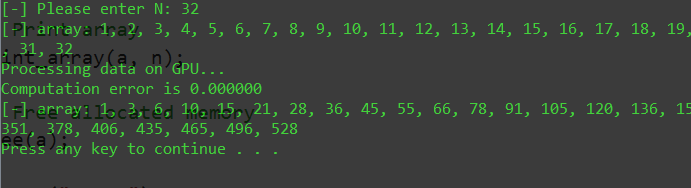
\includegraphics[width=0.7\textwidth]{1_2.png}
	\caption{Computed MSE for Arrays with Size Less than 32.}
	\label{pl1}
\end{figure}

\begin{figure}[!h]\centering
	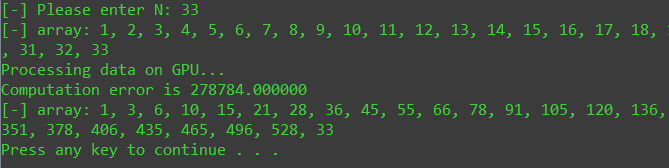
\includegraphics[width=0.7\textwidth]{1_3.png}
	\caption{Computed MSE for Arrays with Size Greater than 32.}
	\label{pl1}
\end{figure}
\newpage
\subsection{Performance Analysis}
Now, let's look at how this implementation performs against the sequential implementation. Table 1.1 illustrates this phenomenon.
\def\arraystretch{1.3}
\begin{table}[!h]
	\centering
	\begin{tabular}{ |p{3cm}||p{3cm}|p{3cm}|p{3cm}|p{2cm}|}

		\hline
		Size & 5 MB & 50 MB & 80 MB &\\
		\hline
		Error   & Very High    & Very High & Very High  & \\
		\hline
		(grid, block)   &  (n/1024, 1024)    &  (n/1024, 1024) &  (n/1024, 1024)&\\
		\hline
		Time(ms)   &   1.285472    &   1.431008 &  1.461440&\\
		\hline
	\end{tabular}
	\caption{Results of Prefix Sum Sequential Implementation of \textit{\textbf{integer}} type.}
	\label{figsolplot}
\end{table}\\
As can be seen from this table, there is a lot of computation error with the raw algorithm of \textit{Hillis \& Steele}. The improvement of the algorithm in next section will solve this problem.

\subsection{A Deeper Look at Blocks and Grids}
Here we'll suppose the array size to be 5 MB only. In this case, there are 1250000 integer elements in the array. Since each multiprocessor can accept up to 1024 threads, we can set the number of blocks to 1221 (Ceil of 1220.70) and the number of threads to 1024 in each block. This solution will not work since the warp size is 32 and there is dependency in different steps of the algorithm. The array will be overwritten and the result is incorrect.

\subsection{Update 1; Minor Improvements}
We can simply scale this implementation by increasing the number of threads per block. We can compute the proper dimensions of \textbf{grid} and \textbf{block} as following:
\begin{cpp}
	// Kernel launch 
	dim3 gridDimensions(ceil((float)n / BLOCK_SIZE), 1, 1);
	dim3 blockDimensions(BLOCK_SIZE, 1, 1);
	
	prefixSumCUDA << < gridDimensions, blockDimensions >> > (d_A, n);
\end{cpp}
This implementation handles input sizes up to \textit{414} elements. Note that \textit{BlockSize} is held 1024 in this case.

\section{Map Reduce Algorithm}
In this implementation which is under \textit{src/normal-implementation}, we have divided the input array into sub arrays. Thus, we have some blocks on the input array which in each block, there are a big number of threads scanning sub arrays. Each of the threads would do multiple additions. Final element of each sub array is finally loaded into another array which holds the last elements of all sub arrays. Then the scan procedure is performed on this array one more time. The results are added back to the elements of the main array respectively.
Note that this implementation handles up to 15000 input sizes which is a massive improvement compared to the initial implementation.
\begin{cpp}
	__global__ void
	prefixSumMap(int *a, int *subArraySumArray, size_t n, size_t k)
	{
		int tId = blockIdx.x * blockDim.x + threadIdx.x;
		
		int startPoint = tId * NUM_OF_ADDS_PER_THREAD;
		int endPoint = startPoint + NUM_OF_ADDS_PER_THREAD;
		
		// Scan sub arrays
		for (int i = startPoint + 1; i < endPoint; i++) {
			
			if (i >= n)
			break;
			
			a[i] += a[i - 1];
		}
		
		__syncthreads();
		subArraySumArray[tId] = a[endPoint - 1];
		
		if (tId == 0) {
			for (int i = 1; i < k; i++) {
				subArraySumArray[i] += subArraySumArray[i - 1];
			}
		}
		
		__syncthreads();
		printf("");
		
		int newStartPoint = startPoint + NUM_OF_ADDS_PER_THREAD;
		int newEndPoint = endPoint + NUM_OF_ADDS_PER_THREAD;
		
		for (int i = newStartPoint; i < newEndPoint; i++) {
			if (i >= n)
			break;
			
			a[i] += subArraySumArray[tId];
		}
	}
\end{cpp}
The greatest bottleneck is when the thread 0 tries to compute the prefix sum of the intermediate array. Also, since \textit{syncthreads} is used to create a synchronization mechanism on the threads of each block, to control other blocks we can buy some time by conducting an \textit{I/O} instruction. Note that we haven't taken care of the timings in this implementation.

\section{Brent Kung Scan with Arbitrary Size Support }
This implementation supports input arrays with arbitrary size. It includes 3 main steps(kernels):
\begin{itemize}
	\item Scan sub arrays of the input array with normal approach
	\item Scan the intermediate array with Brent Kung approach
	\item Reduce the result back to the main array
\end{itemize}

\subsubsection{Source Code}
Various implementations are attached in the \textit{src} folder. This implementation is under \textit{final-implementation} subdirectory.

\subsubsection{Serial vs Parallel Timings}

\subsubsection{Grid Size \& Block Size Analysis}
Maximum number of blocks and their sizes is heavily dedicated to the GPU model. The important thing about this implementation is that, whenever a single thread does less computations (smaller sub array size), the performance gets better. For the input of size $n$, each thread scans a sub array with size \textit{NUM\_OF\_ADDS\_PER\_THREAD}. The block size should be a coefficient of the job size each thread is working on. Maximum block size is 1024 for compute capability of 5 in \textit{x} direction. Thus, the proper grid size (which is the number of blocks) is \textit{ceil((float) n / BLOCK\_SIZE)}. For larger input sizes, the value of \textit{NUM\_OF\_ADDS\_PER\_THREAD} should be increased for the computation to be error prone.
\begin{figure}[!h]\centering
	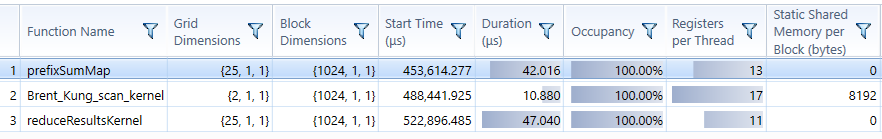
\includegraphics[width=0.75\textwidth]{3_1.png}
	\caption{Summary of Grid and Block Sizes of 3 Kernels.}
	\label{pl1}
\end{figure}
Figure 3.2 illustrates the total occupancy. It also demonstrates that the number of blocks, which is 2 in this case, is the cause of occupancy limit.
\begin{figure}[!h]\centering
	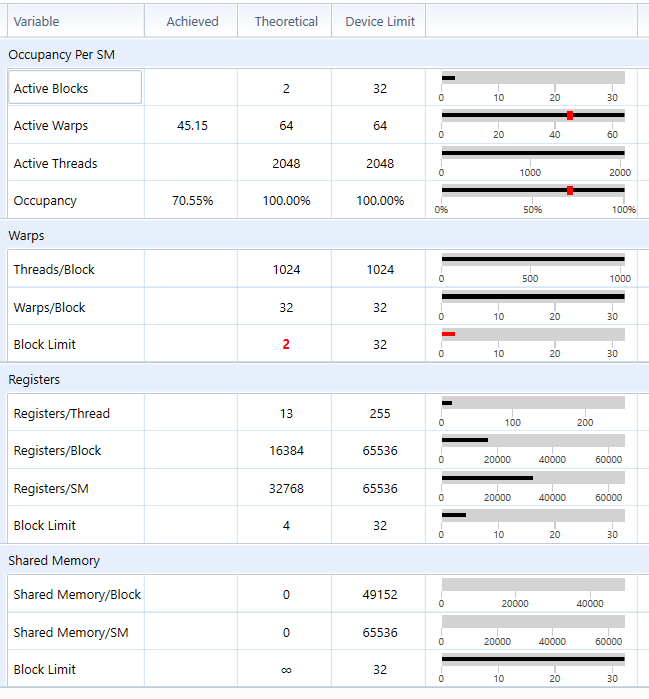
\includegraphics[width=0.55\textwidth]{3_2.png}
	\caption{Experimental Results of Occupancy of \textit{PrefixSumMap} Kernel.}
	\label{pl1}
\end{figure}
\newpage
Figure 3.3 shows how much time is wasted for global memory accessing. It clearly depicts the issue stall reasons for the \textit{PrefixSumMap} kernel.

\begin{figure}[!h]\centering
	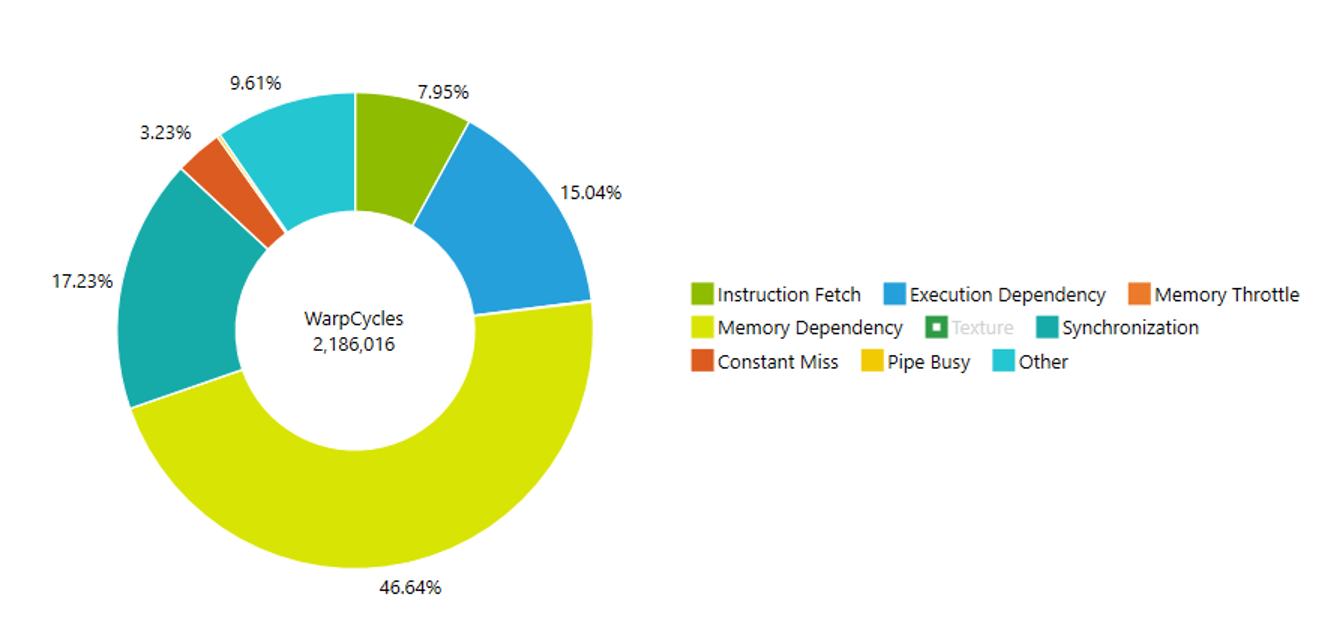
\includegraphics[width=0.55\textwidth]{3_3.png}
	\caption{Issue Stall Reasons of \textit{PrefixSumMap} Kernel.}
	\label{pl1}
\end{figure}

\subsubsection{SM Activity Analysis}
Figure 3.4 shows the percentage of time each multiprocessor was active during the duration of the kernel launch. A multiprocessor is considered to be active if at least one warp is currently assigned for execution. An SM can be inactive - even though the kernel grid is not yet completed - due to high workload imbalances. Such uneven balancing between the SMs can be caused by a few factors: Different execution times for the kernel blocks, variations between the number of scheduled blocks per SM, or a combination of the two.
\begin{figure}[!h]\centering
	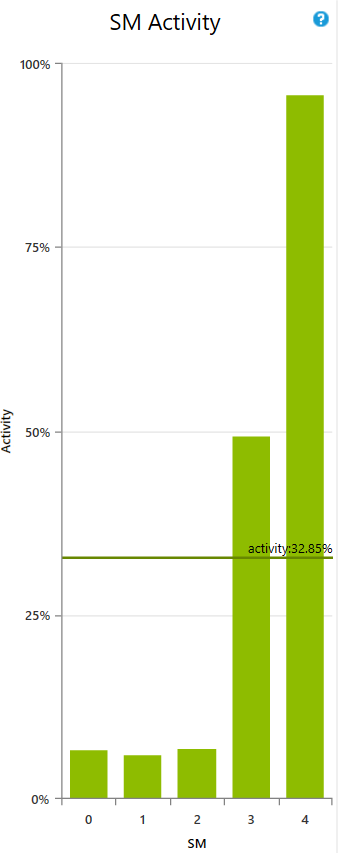
\includegraphics[width=0.2\textwidth]{3_4.png}
	\caption{SM Activity of \textit{PrefixSumMap} Kernel.}
	\label{pl1}
\end{figure}
\end{document}

